
\documentclass[a4paper,12pt]{report}
%    \renewcommand{\baselinestretch}{1.6}      % interline spacing
%
% \includeonly{}
%
%			PREAMBOLO
%
\usepackage[a4paper]{geometry}
\usepackage{amssymb,amsmath,amsthm}
\usepackage{graphicx}
\usepackage{url}
\usepackage{hyperref}
\usepackage{epsfig}
\usepackage[italian, english]{babel}
\usepackage{setspace}
\usepackage{tesi}
\graphicspath{ {./img/} }
\usepackage{float}


% per le accentate
\usepackage[utf8]{inputenc}
%
\newtheorem{myteor}{Teorema}[section]
%
\newenvironment{teor}{\begin{myteor}\sl}{\end{myteor}}
%
%
%			TITOLO
%
\begin{document}

  

\title{Cloud Gaming}
\author{Daniele Bocchino}
\anno{2021-2022}
\matricola{991031}
\relatore{Prof. Gianini Gabriele}


\beforepreface
\textbf{}
\afterpreface
%
%
%			
\chapter{Introduction}
\label{cap1}
%
%
\section{Cloud Gaming}
During the Covid-19 pandemic of 2020, a lot of people were forced to stay at home for several month and  a lot of them looked for a different way to spend their time. New people have entered the world of video games and they tried to purchase the best solution for playing games. Unfortunately due to the chip crisis and production slowdowns caused by the pandemic to purchase a console or built PC games had became a titanic challenge. For this reason a lot of people has opted for cloud-based solutions to play major video game titles.\\
%
\paragraph{History of Cloud Gaming\\\\}
The first approach of cloud gaming technology sates back to the early 2000s. For several years this technology didn't explode due by lower connection performance  and other problems. Recently, after explosion of various SaaS ( Software as a Service ) such as Netflix, and access to a fast internet connection for many people, more and more companies have wanted to invest in the cloud-based gaming. Large Company such as Google, Amazon, Microsoft, Nvidia, Shadow, etc... Have invested in the possibility of playing video games in the cloud.\\

%
\paragraph{How could gaming really works?\\\\}
Cloud gaming allows users to play online games through remote hardware owned by a cloud provider. Instead of players inserting a game disc into a gaming console or downloading a game’s file to their device, players stream games via the web. This solution allow anyone with a good connection to play the best games in the world ( the classic games called AAA ) with any type of device that can be connected to the internet.\\\\
The idea is really great, allowing gamers not to buy a specific device and play the best games on smartphones, tablets or computers without incredible performance. \\
%
Cloud gaming platforms works as a remote desktop. The games are stored and executed on remote computer, and then streamed on the player's device. In many case, users are required to download a specific application or navigate to a dedicated web page to start playing games. Through this method the users don't have to worry about downloading games, updating it or upgrading hardware. This operation are managed by service provider.\\\\
%
In addition to taking care of the hardware, the service provider also takes care of adding new games; in fact, a different cloud games provider offers a monthly subscription that includes a library with some available games. In general this game are of different types and popularity. \\\\
%
\paragraph{Advantages of Cloud Gaming\\\\}

The cloud gaming has brought a plethora of benefits to users and the gaming world, first and foremost the ability to play a large number of titles without  expensive hardware and on any type of devices. Other advantages are related to the ability to try a lot of games without purchasing them and reduce time it takes users to update and download the games. In fact, to play on cloud, users need nearly 20 Mb/s download connection ( this value depends on the desired image resolution and the type of service provider). At this speed, it may take several hours to download the game. 
%
\paragraph{Disadvantages of Cloud Gaming\\\\}
Cloud gaming doesn't only have advantages, with this immature technology there are some disadvantages that may disappoint the most demanding gamers. The main problem with this type of gaming is the connection, although many people connect with a very fast internet ( the famous gigabit connection ) this type of technology depends on latency. In fact in many cases, the very fast internet connection is not enough for a great cloud gaming experience. For this reason in a lot of games that the timing and precision of the users input is mandatory for obtain a really good experience ( such as First-person shooters and fighting games) will not work as a local machine and the user experience will be sacrificed. Another disadvantage is related to the game library, a problem that depends on the service provider and the relationship between the service provider and game companies. It may indeed be the case that a recent game needs a few months before it becomes available on the on-demand library, or it is possible that a game will never be available. 
 %
\chapter{Process}
\label{cap2}
\section{The Users}
As in any business, everything revolves around customers, Cloud Gaming was created for them, to offer a viable alternative to traditional gaming. It is a great solution for off-site students, commuters and all those people who do not need very high performance with some small sacrifices. \\
Users are required to register and pay a monthly subscription for to use the service.  Depending on the Cloud gaming service provider the users can use the service on web browser or on dedicated application. After logging in the user can choose the game he wants and start it. 
If the user wishes, he/she can terminate the subscription at any time and reactivate it whenever he/she wants. 
%
\section{The Cloud computing service }
A cloud computing service is a service that allows users to play a large number of games. This is done by providing enough high-performance hardware to support the load of users and enjoy the service to the fullest.  The company providing this service includes different types of workers. In this project, it is assumed that the part of the company providing the service includes the financial team, the support team and the engineering team.
%
\subsection{The support team }
The support team is a group of people who interface with customers. In general, this team monitors orders, provides access to users, responds to customer problems, and provides support.
%
\subsection{The engineering team }
The engineering team is a group of people who work with the machines. In general, this team monitors machine, fix problem, make upgrade to hardware, manage all dates inside the cloud etc... they are in charge of making the games available in the cloud after receiving them from the manufacturing companies following the agreements between the two parties.
%
\subsection{The financial and Management team }
The finance and management team is a group of people who interface with video game companies. Their goal is to discuss with video game companies to obtain permission to distribute the game on the cloud platform in exchange for payment.  
%
\section{The video game company  }
A video game company  is a company that create video games. Often these video games are only available on certain platforms or certain devices ( such as console exclusives ). In the specific case examined by this project, the video game company interfaces with the company that provides a could computing service to make its products available on the cloud gaming library. This company is composed by different department. In this project, it is assumed that the  company includes Design Department, Development Department, Release and Management Department
%
\subsection{Development Department }
It is the department of a video game company that deals with the development part of a new game, the creation of new features, and the fixing of structural bugs in the video game.
%
\subsection{Release and Management Department }
It is the department of a video game company that deals with the release part of a new game. It interfaces with the financial and management team of the company that runs the cloud computing service. His job is to sell the product to the cloud computing company at the best price and then provide the engineering team with the product to be able to put into the on demand library.
%
%
\chapter{Business Process Flow}
\section{BPMN - Business Process Model and Notation Diagram }
Business Process Model and Notation (BPMN) is a graphical representation for specifying business processes in a business process model.\\
Business Process Model and Notation(BPMN) is a standard for business process modeling that provides a graphical notation for specifying business processes in a Business Process Diagram (BPD).\\
The objective of BPMN is to support business process management, for both technical users and business users, by providing a notation that is intuitive to business users, yet able to represent complex process semantics.\\
The BPMN specification also provides a mapping between the graphics of the notation and the underlying constructs of execution languages, particularly Business Process Execution Language (BPEL).
\section{Full Diagram}
\begin{figure}[H]
 \centering
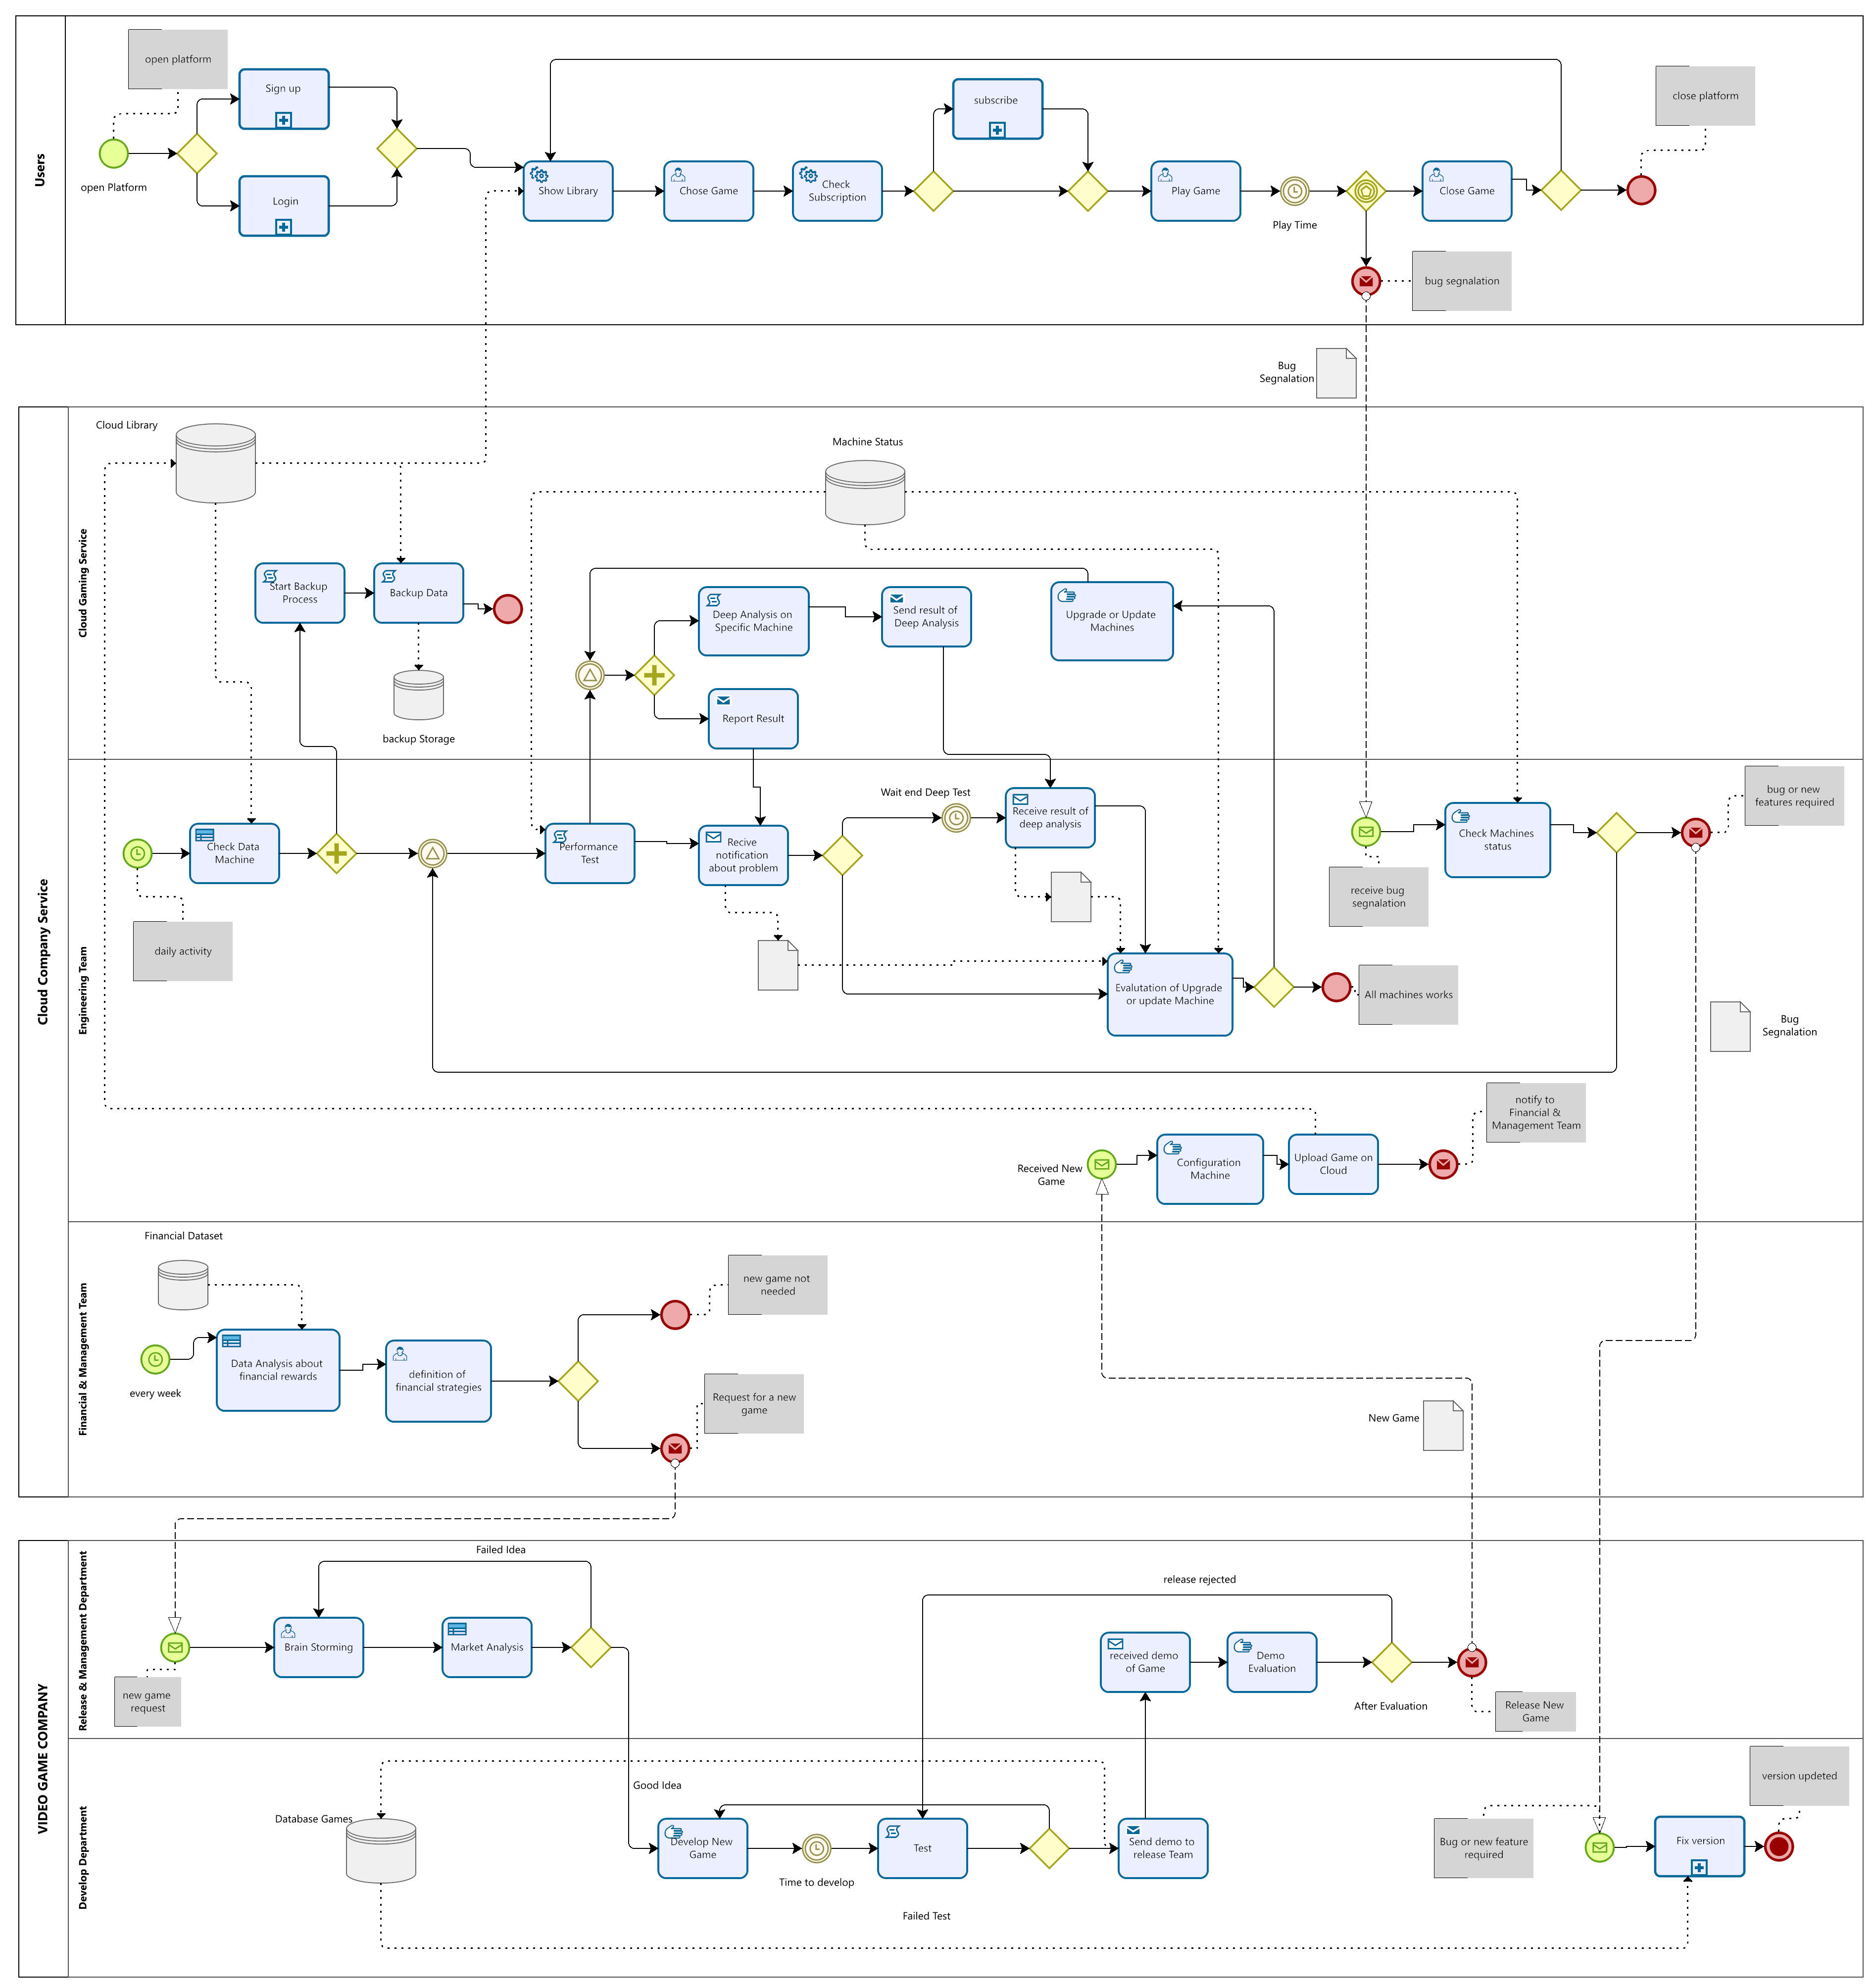
\includegraphics[scale=0.15]{Full_BPMN}
\caption{Full BPMN Diagram}
\label{FULL BPMN}
\end{figure} 
%
%
\section{The Users}
\begin{figure}[H]
 \centering
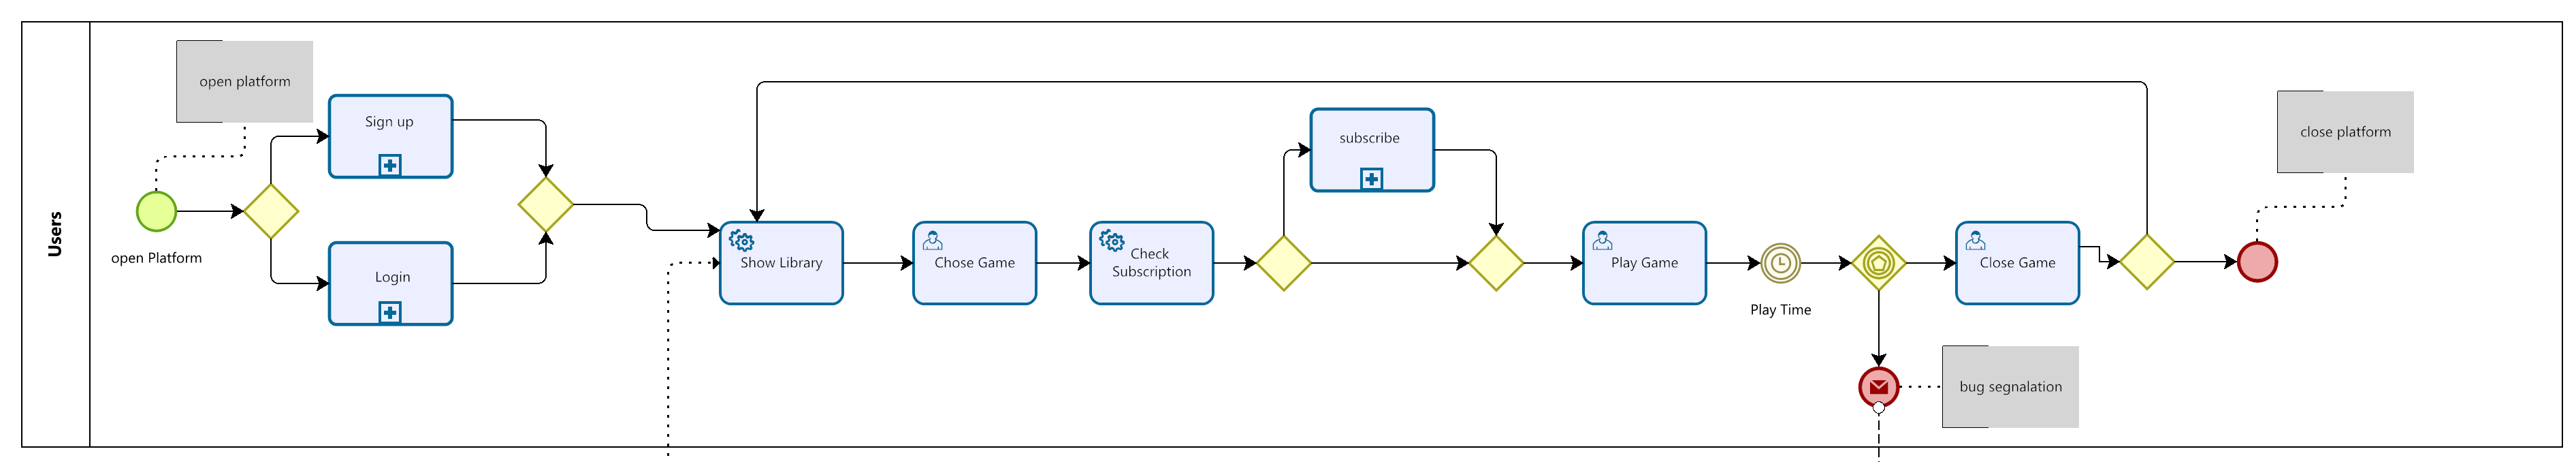
\includegraphics[scale=0.16]{user_BPMN}
\caption{Users BPMN Diagram}
\label{Users BPMN}
\end{figure} 

\subsection{Sub Process - Login }
\begin{figure}[H]
 \centering
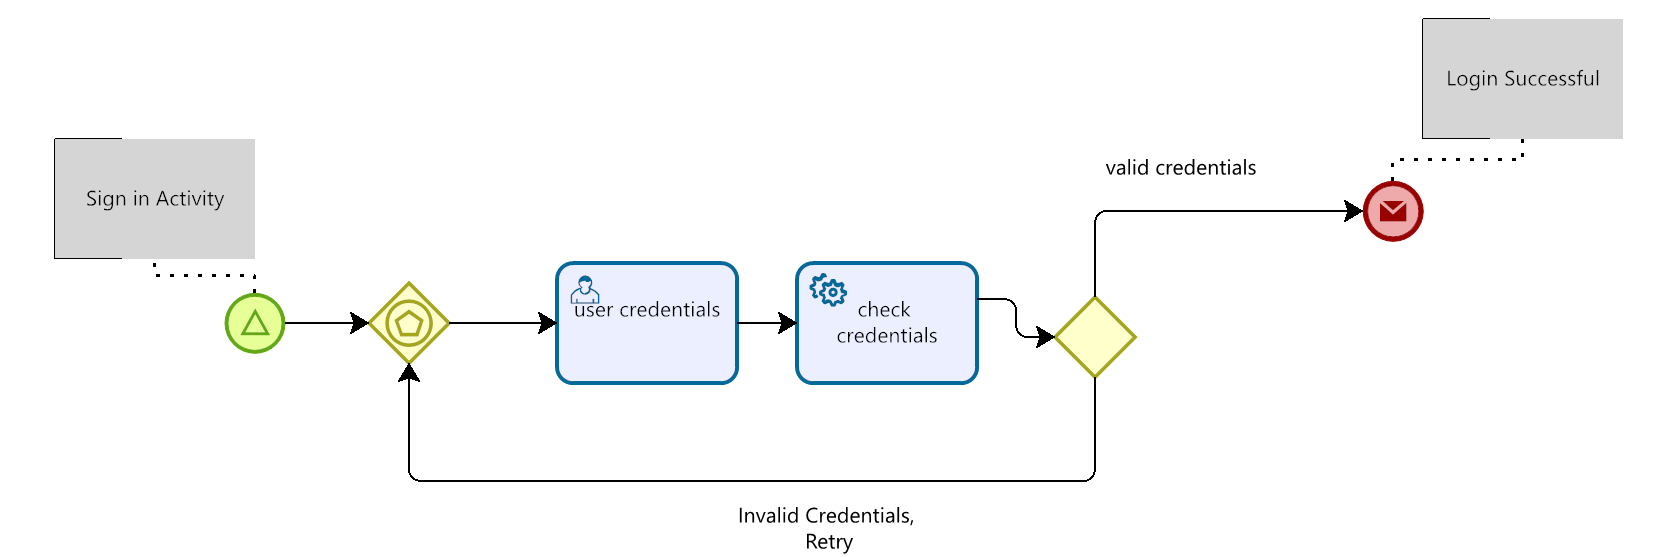
\includegraphics[scale=0.35]{login_BPMN}
\caption{Sub Process - Login BPMN Diagram}
\label{Login BPMN}

\end{figure} 

\subsection{Sub Process - Register }
\begin{figure}[H]
 \centering
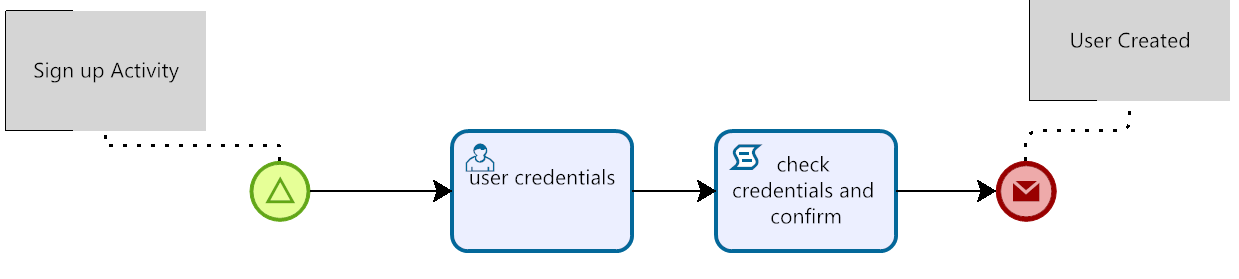
\includegraphics[scale=0.35]{signup_BPMN}
\caption{Sub Process - Sign up BPMN Diagram}
\label{Signup BPMN}
\end{figure} 

\subsection{Sub Process - Subscription }
\begin{figure}[H]
 \centering
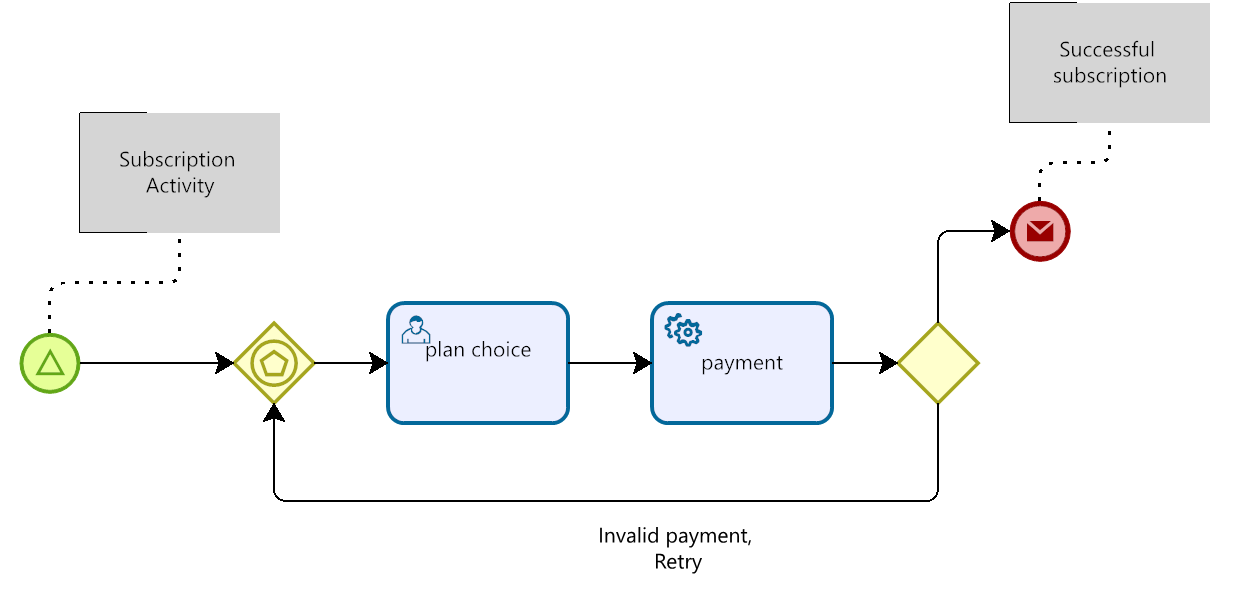
\includegraphics[scale=0.35]{subscription_BPMN}
\caption{Sub Process - Subscription BPMN Diagram}
\label{Subscription BPMN}
\end{figure} 

\section{The Cloud Computing service }
\begin{figure}[H]
 \centering
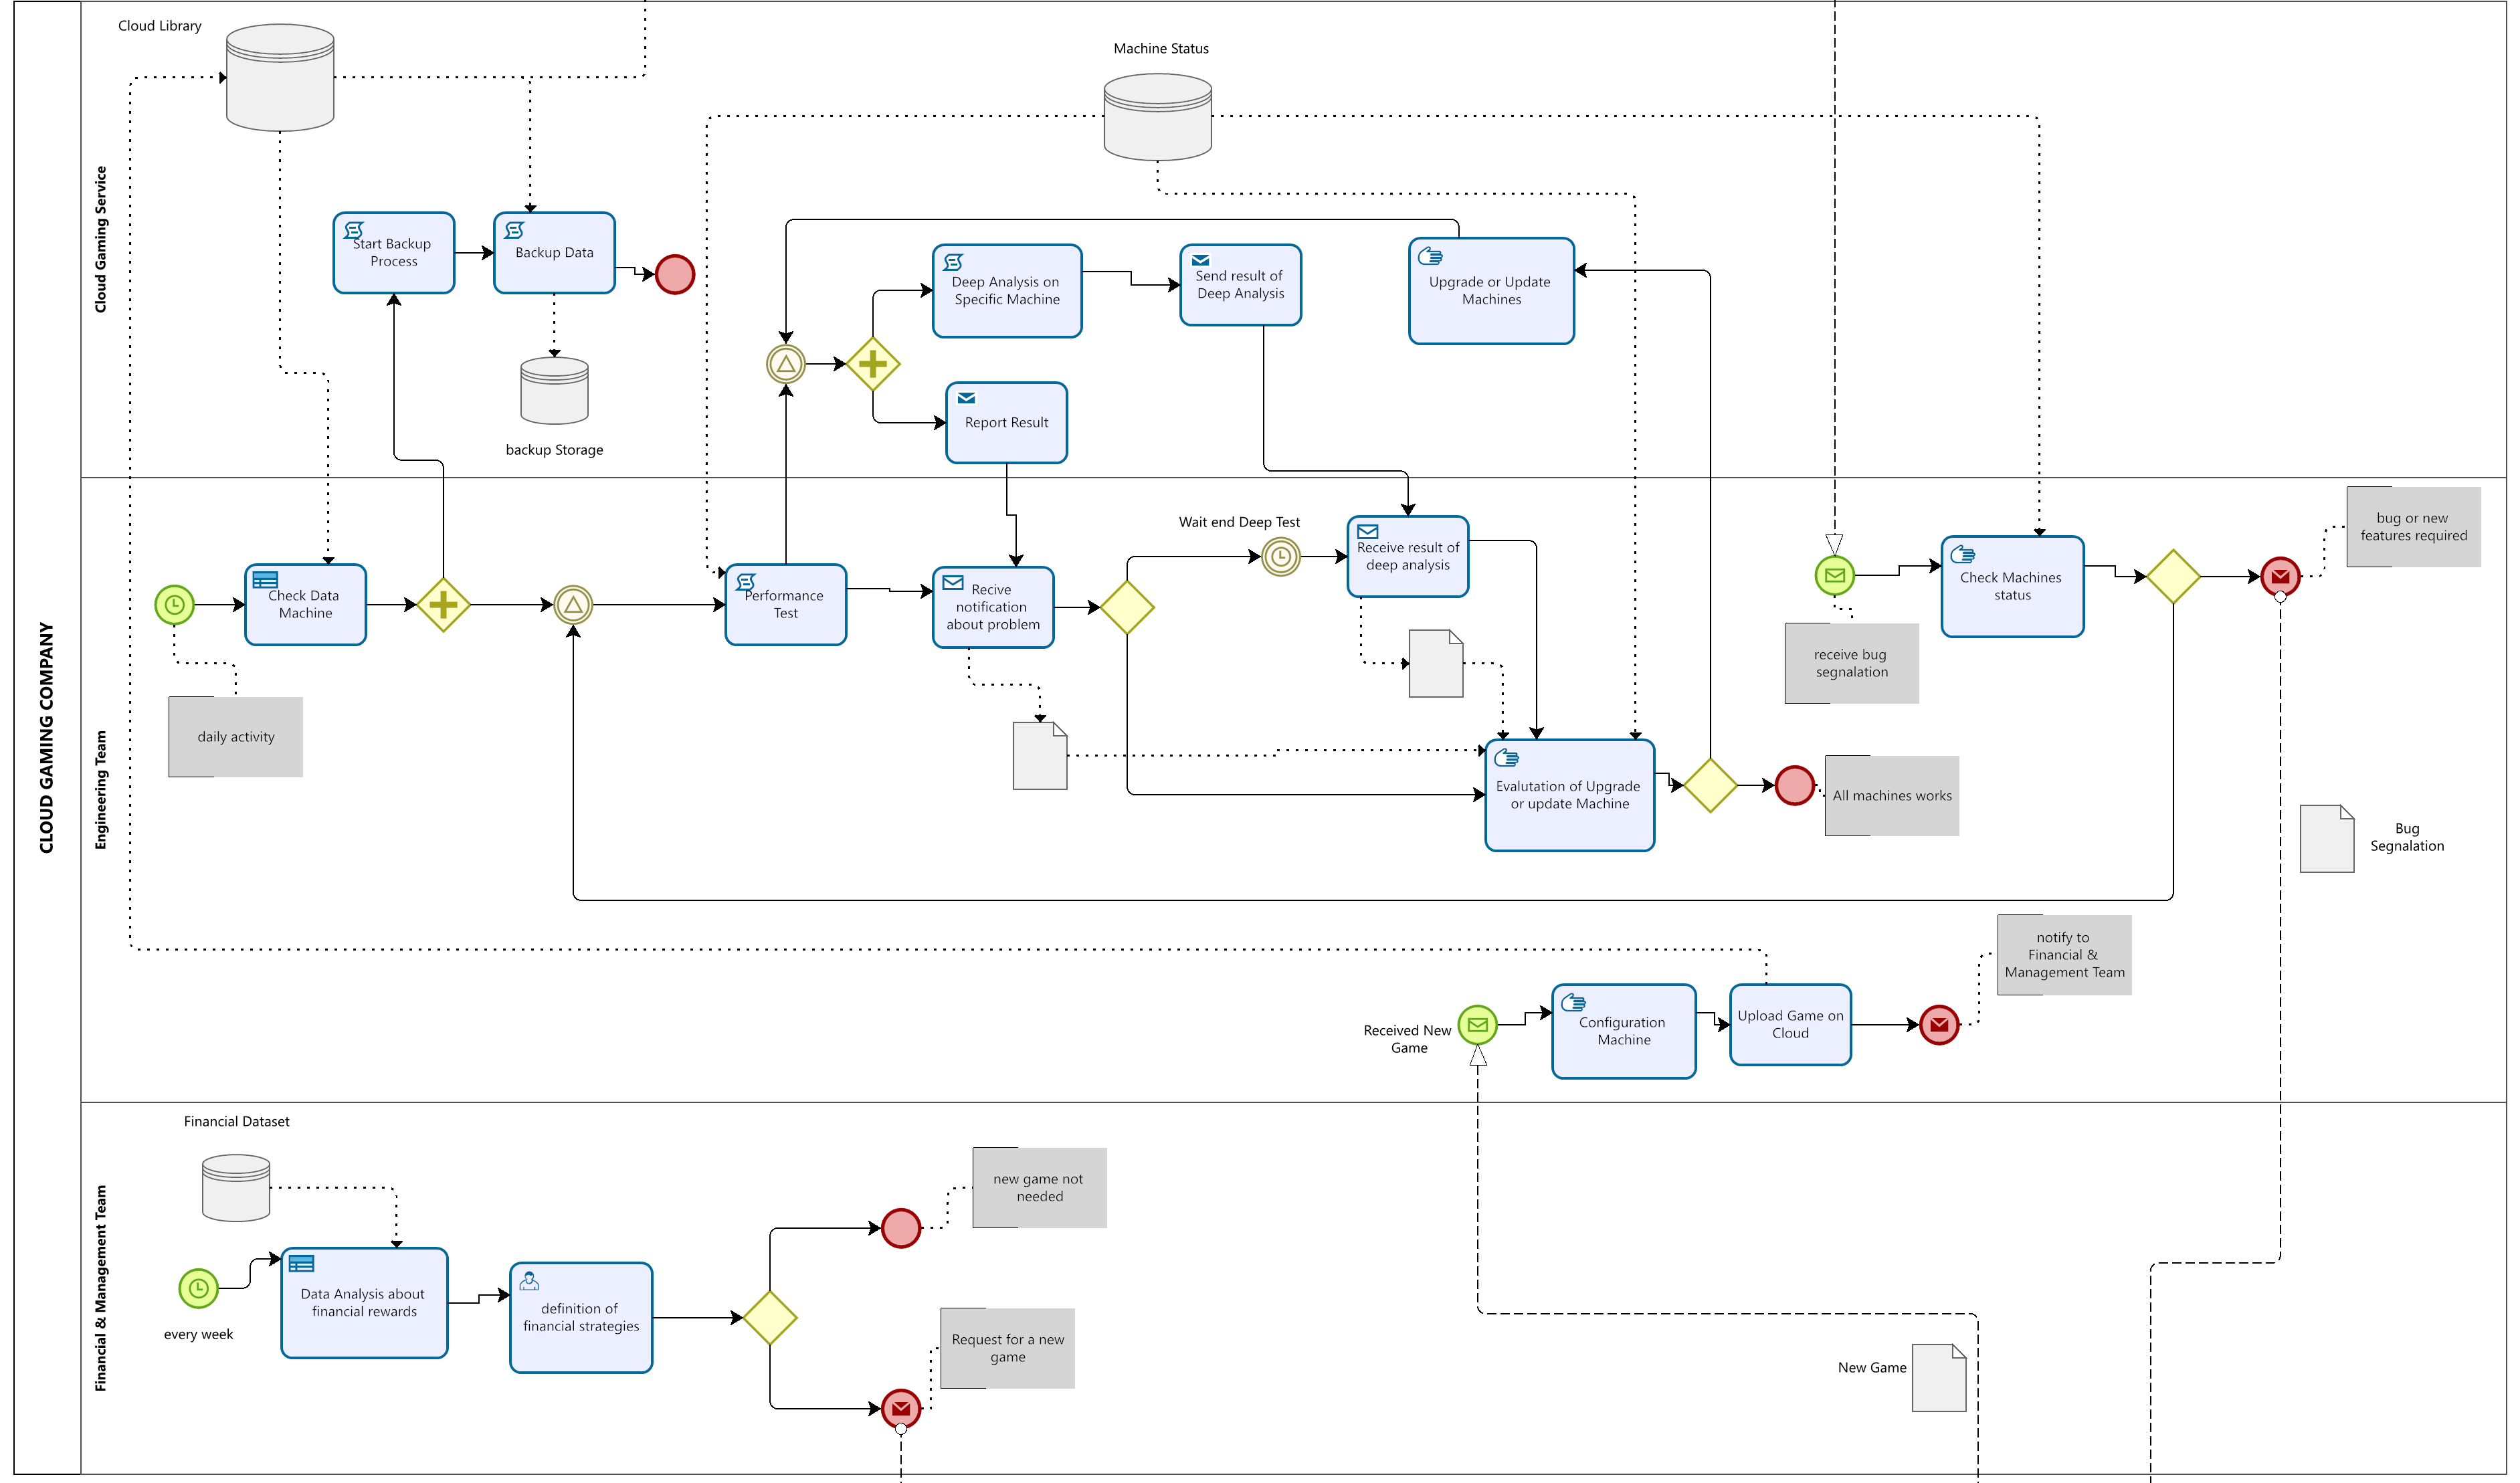
\includegraphics[scale=0.15]{cloud_BPMN}
\caption{Cloud Computing Service BPMN Diagram}
\label{Cloud BPMN}

\end{figure}



\section{The video game company  }
\begin{figure}[H]
 \centering
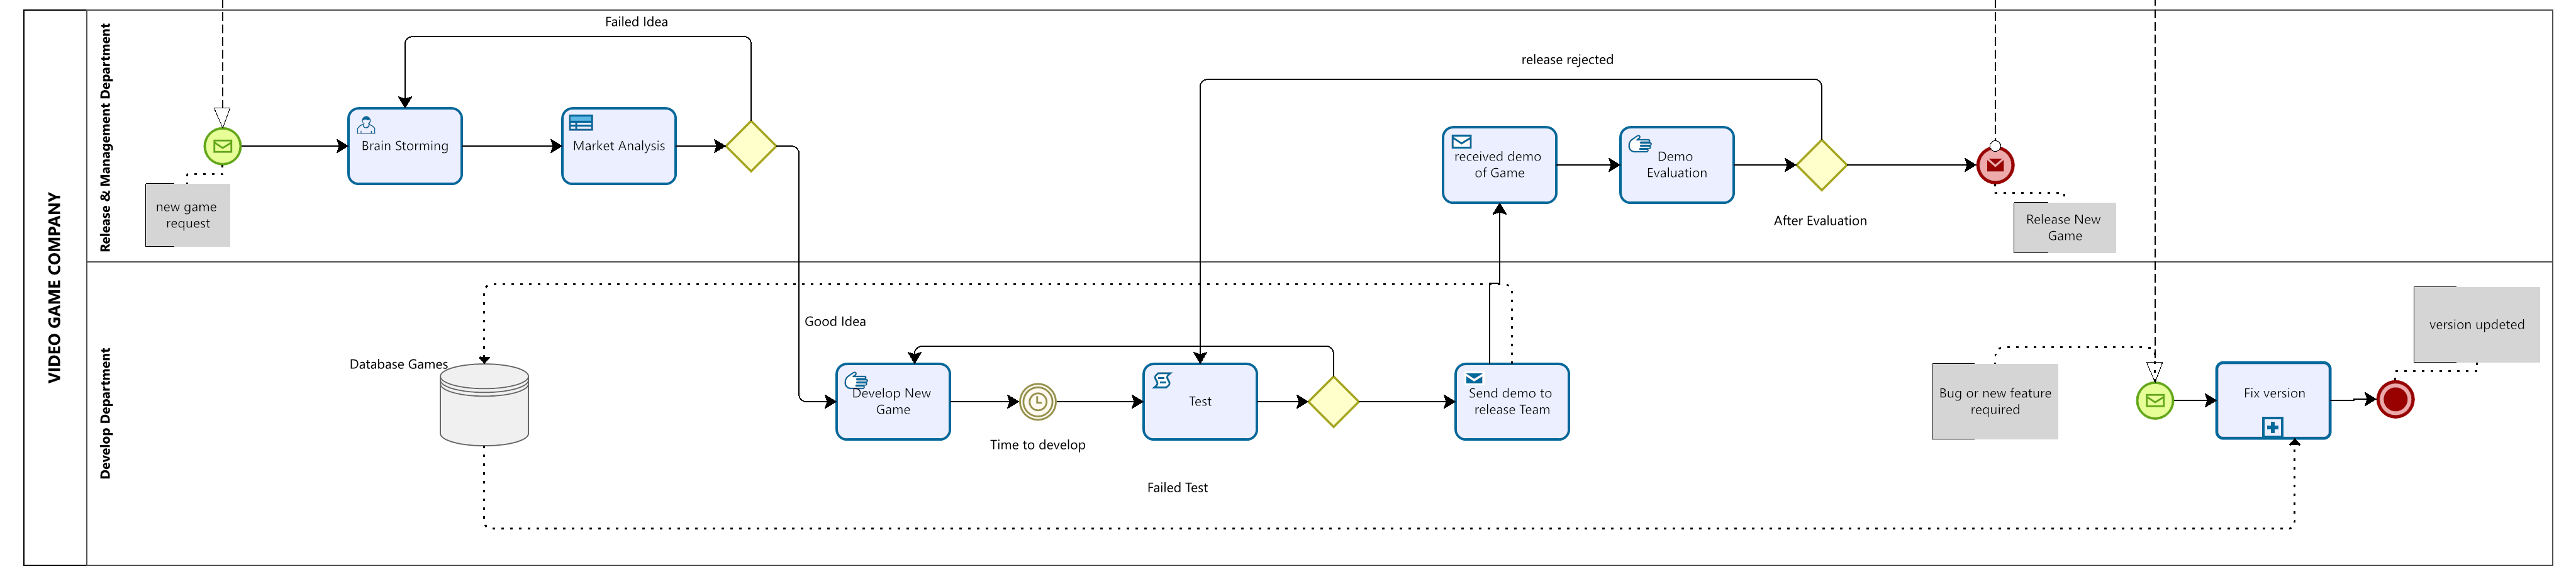
\includegraphics[scale=0.15]{videogame_BPMN}
\caption{Video Game Company BPMN Diagram}
\label{VideoGame BPMN}
\end{figure} 

\subsection{Sub Process - Fix Version }
\begin{figure}[H]
 \centering
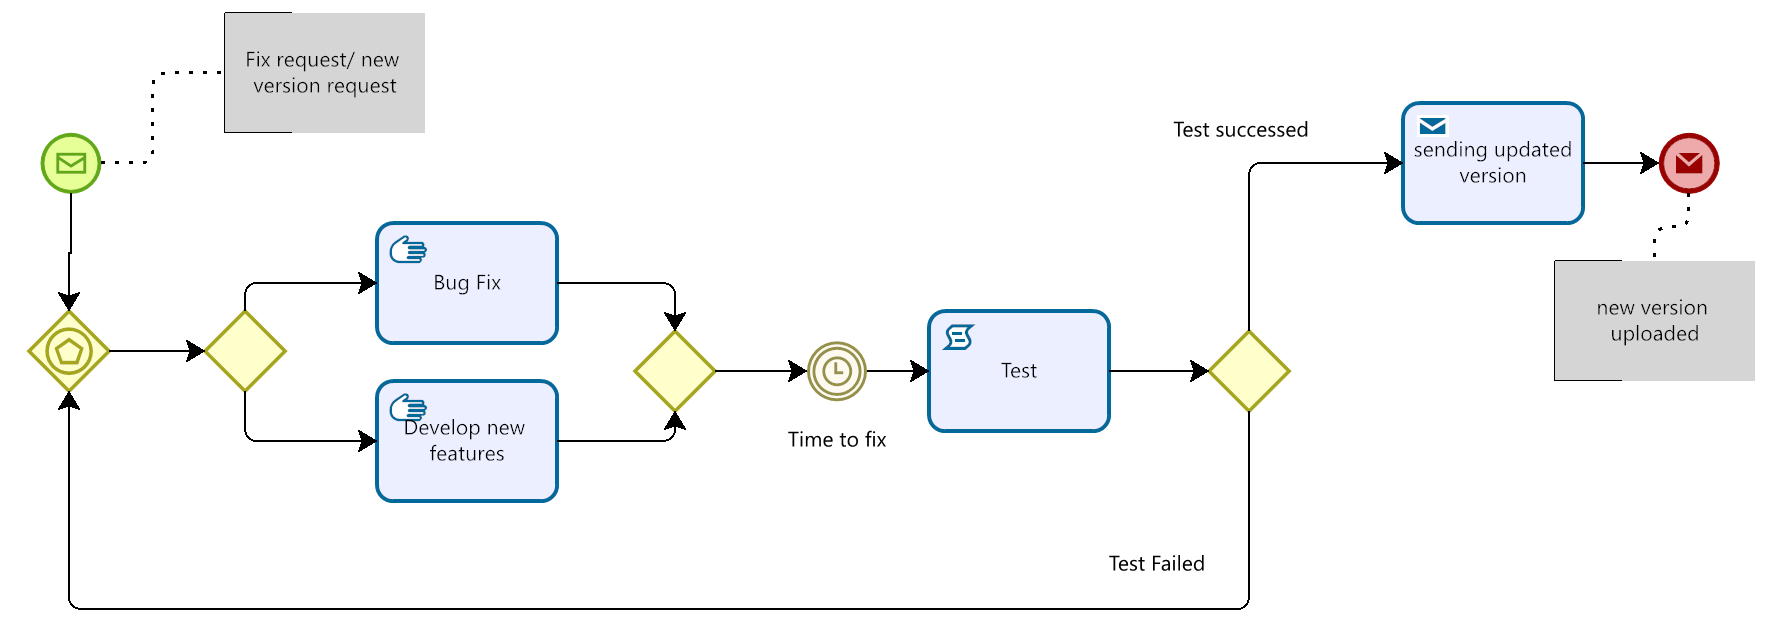
\includegraphics[scale=0.35]{developer_BPMN}
\caption{Sub Process - Fix Version BPMN Diagram}
\label{Fix Version BPMN}

\end{figure} 

\chapter{Value Model}
The Value Model describes what constitutes value in an organisation, where organisations create value, how stakeholders exchange value, and more importantly, how an organisation can find new opportunities to create value.

\section{Actor}

\paragraph*{Users}
\begin{itemize}
\item{\textbf{Users:} Market segment actor using the cloud platform in return for payment.
Users can play on the platform any game made available by the cloud computing service.} 
%
\end{itemize}
%
%
\paragraph*{Cloud Gaming Service}
\begin{itemize}
\item{\textbf{Cloud Gaming Service:} Actor referring to the cloud gaming platform.
This platform contains the games uploaded by the engineering team. This team is also responsible for the maintenance of the platform. Users can register and use the platform. } 
%
\item{\textbf{Engineering Team:}  Actor referring to the engineering team.
The ignegneri team works for the cloud gaming service, they monitor the platform, perform maintenance, update and add new content, and operate in case there are bugs on the service. } 
%
\item{\textbf{Financial \& Management Team:}  Actor referring to the Financial \& Management team.
This team is in charge of checking the performance of the platform in terms of economics, evaluating data, and requesting new content from the Video Game company. } 
%
\end{itemize}
%
%
\paragraph*{Video Game Company}
\begin{itemize}
\item{\textbf{Develop Department:} Actor who is part of the video game company.
His job is to release new games defined by the Release \& Management department. It is also in charge of updating existing games and making bug fixes when they are reported } 
%
\item{\textbf{Release \& Management Department:}  Actor who is part of the video game company.
His job is to communicate with the Financial \& Management Team to define new games and analyze their cost. In addition to the business aspect, he is in charge of releasing the game as a result of the request from the cloud gaming service to have a new content on the platforms.
} 
\end{itemize}
\section{Value Diagram}

\begin{figure}[H]
 \centering
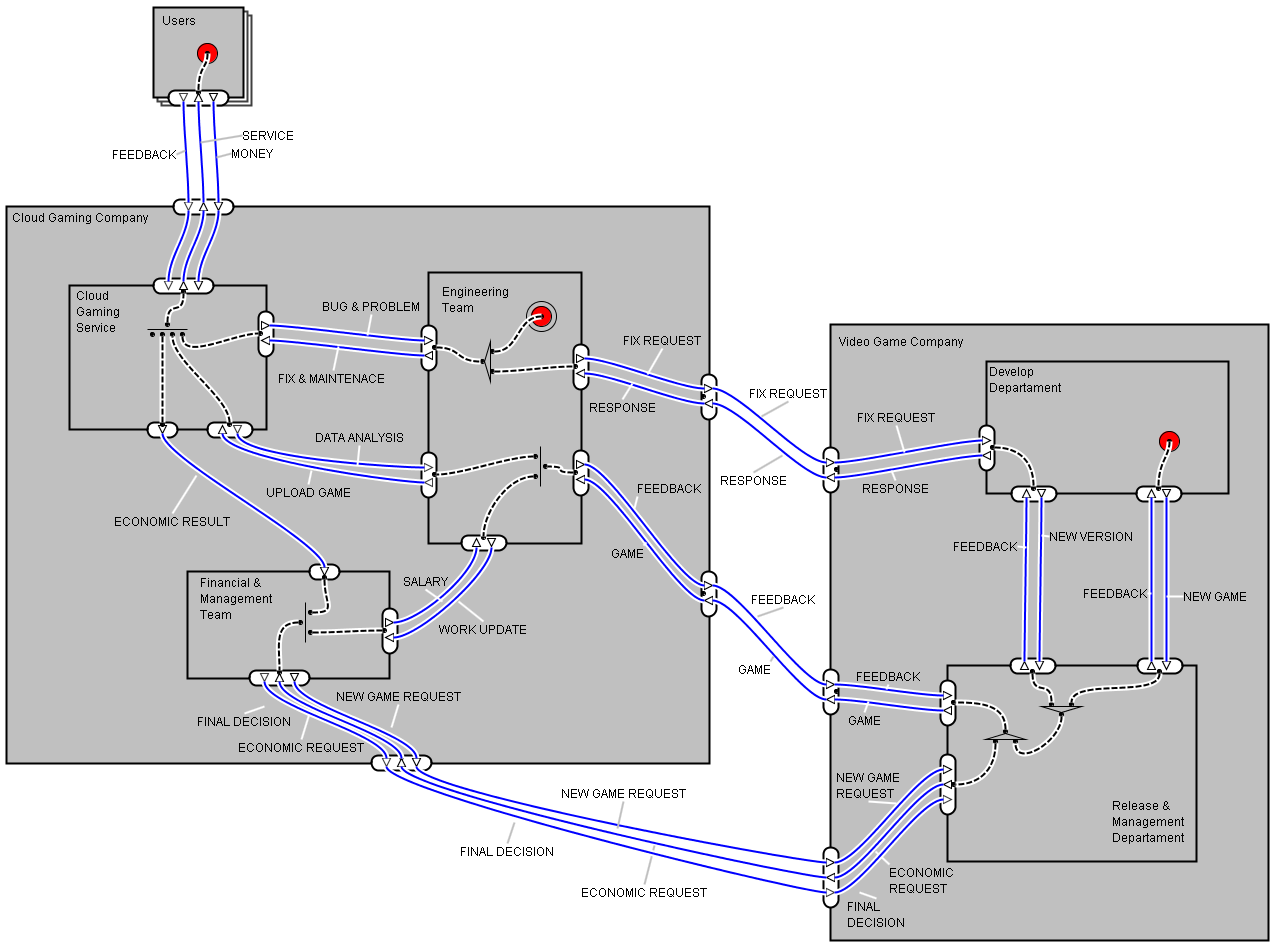
\includegraphics[scale=0.45]{value_model}
\caption{Value Diagram}
\label{Value Diagramn }
\end{figure} 

\chapter{Business Evaluation}
\section{Critical Successor Factors (CSF)}
\section{Key Goal Indicators}
\section{Key Performance Indicators}
The Key Performance Indicators (KPIs) allows to measure the success factors represented by the
different activities, in particular they allow to verify if the activity is carried out properly and to
determine the "bottlenecks" of the system.
\begin{itemize}
\item{Rate of Addition of new users - Number of Active users in the platform}
\item{ Ratio of Items/Lessee - Rate of Items available for lending}
\item{Average Density of Items - Availability of items over the serviceable area}
\item{ Average Wait time - time from submission of request to completion.}

\end{itemize}

\section{KPI in Practice}
TABELLAAA!!!
\chapter{Conclusion}
The initial objective has been reached: the operation of the company has been correctly modeled
and this has allowed us to identify the factor required for a steady growth of the company. Thanks
to CSFs and KPIs it was possible to identify the best strategy to speed up the times and identify the
most suitable elements and time slots to achieve this purpose. Furthermore the realized BPMNs have
allowed us to understand in a simple but elective way the carrying out of the various processes even
for non-experts in the eld.
\end{document}


 
